\section{Generowanie grafów}

\subsection{Generowanie grafów nieizomorficznych} 

\begin{algorithm}
  \caption{Generowanie grafów nieizomorficznych}
  \begin{algorithmic}
  \REQUIRE $n > 0 $
  \STATE grafy[] <- graf jednowierzchołkowy 
  \WHILE{$ilośćWierzchołków(grafy) < n$}
    \STATE dodajWierzchołek(grafy)
    \STATE usunIzomorfizmy(grafy)
  \ENDWHILE
  \end{algorithmic}
\end{algorithm}

W uproszczeniu: generowanie grafów rozpoczynamy od pojedynczego wierzchołka.
Następnie powtarzamy następujące kroki dopóki nie osiągniemy docelowej liczby wierzchołków:
\begin{enumerate}
 \item Generowanie grafów nieizomorficznych 

 \begin{itemize}
 \item  Dodanie nowego wierzchołka  

 \item Utworzenie wszystkich możliwych zestawów krawędzi zawierających ten wierzchołek. Przy dodawaniu n-tego wierzchołka mamy 

 \item Sprawdzenie izomorfizmów - jeżeli wygenerowany graf jest izomorficzny z innym wygenerowanym grafem, to pozostawiamy tylko jeden z nich 
 
 \end{itemize}
\end{enumerate}

Zaczynamy od pojedynczego wierzchołka.

\begin{figure}[H]
  \centering
  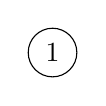
\begin{tikzpicture}[node distance={15mm}, main/.style = {draw, circle}] 
    \node[main] (1) {$1$};
   \end{tikzpicture}
   \caption{}
\end{figure}

\begin{figure}[h]
  \centering
  \begin{tikzpicture}[node distance={15mm}, main/.style = {draw, circle}] 
    \node[main] (2) [below of=1] {$1$};
    \node[main] (3) [right of=2] {$2$};
   
    \node[main] (4) [right of=3] {$1$};
    \node[main] (5) [right of=4] {$2$};
   
    \draw (2) -- (3);
   \end{tikzpicture}
   \caption{}
\end{figure}

W pierwszym kroku dodajemy drugi wierzchołek i otrzymujemy dwa różne grafy - jeden, w którym wierzchołki sąsiadują, drugi, w którym nie. 

\begin{figure}[H]
  \centering
  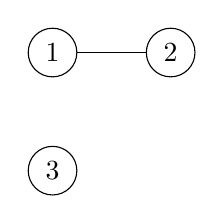
\begin{tikzpicture}[node distance={15mm}, main/.style = {draw, circle}] 
    \node[main] (1) {$1$};
    \node[main] (2) [right of=1] {$2$};
    \node[main] (3) [below of=1] {$3$};
   
    \draw (1) -- (2);
   \end{tikzpicture} 
   \hfill
   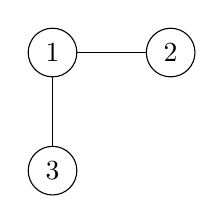
\begin{tikzpicture}[node distance={15mm}, main/.style = {draw, circle}] 
    \node[main] (1) {$1$};
    \node[main] (2) [right of=1] {$2$};
    \node[main] (3) [below of=1] {$3$};
   
    \draw (1) -- (2);
    \draw (1) -- (3);
   \end{tikzpicture} 
   \hfill
   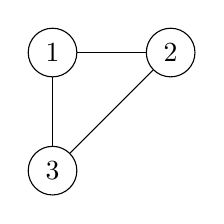
\begin{tikzpicture}[node distance={15mm}, main/.style = {draw, circle}] 
    \node[main] (1) {$1$};
    \node[main] (2) [right of=1] {$2$};
    \node[main] (3) [below of=1] {$3$};
   
    \draw (1) -- (2);
    \draw (1) -- (3);
    \draw (2) -- (3);
   \end{tikzpicture} 
  
  \caption{Grafy wygenerowane z pierwszego grafu z poprzedniego kroku}
\end{figure}

Następnie bierzemy pierwszy z grafów i dodajemy do niego kolejny wierzchołek, ponownie generując wszystkie możliwości.  

\begin{figure}[H]
  \centering
  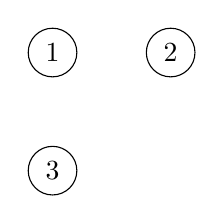
\begin{tikzpicture}[node distance={15mm}, main/.style = {draw, circle}] 
  \node[main] (1) {$1$};
  \node[main] (2) [right of=1] {$2$};
  \node[main] (3) [below of=1] {$3$};

  \end{tikzpicture}
  \hfill
  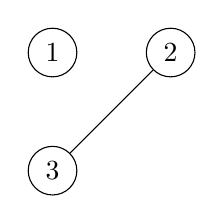
\begin{tikzpicture}[node distance={15mm}, main/.style = {draw, circle}] 
  \node[main] (1) {$1$};
  \node[main] (2) [right of=1] {$2$};
  \node[main] (3) [below of=1] {$3$};

  \draw (3) -- (2);
  \end{tikzpicture}
  \hfill
  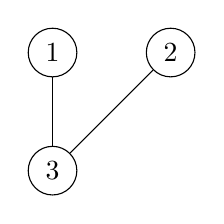
\begin{tikzpicture}[node distance={15mm}, main/.style = {draw, circle}] 
  \node[main] (1) {$1$};
  \node[main] (2) [right of=1] {$2$};
  \node[main] (3) [below of=1] {$3$};

  \draw (3) -- (2);
  \draw (1) -- (3);
  \end{tikzpicture}
  \caption{{Grafy wygenerowane z drugiego grafu z poprzedniego kroku}}
\end{figure}

To samo powtarzamy dla grafu drugiego. 

Jak łatwo zauważyć graf 1 i graf 5 oraz graf 2 i graf 6 są parami izomorficzne, więc możne odrzucić po jednym z każdej pary, zmniejszając liczbę grafów rozważanych w kolejnych krokach.  

\begin{figure}[H]
  \centering
  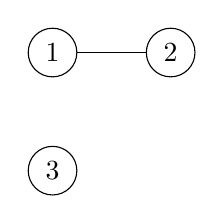
\begin{tikzpicture}[node distance={15mm}, main/.style = {draw, circle}] 
    \node[main] (1) {$1$};
    \node[main] (2) [right of=1] {$2$};
    \node[main] (3) [below of=1] {$3$};
   
    \draw (1) -- (2);
   \end{tikzpicture} 
   \hfill
   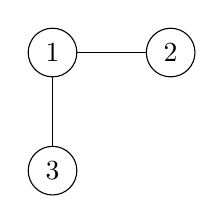
\begin{tikzpicture}[node distance={15mm}, main/.style = {draw, circle}] 
    \node[main] (1) {$1$};
    \node[main] (2) [right of=1] {$2$};
    \node[main] (3) [below of=1] {$3$};
   
    \draw (1) -- (2);
    \draw (1) -- (3);
   \end{tikzpicture} 
   \hfill
   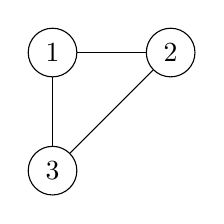
\begin{tikzpicture}[node distance={15mm}, main/.style = {draw, circle}] 
    \node[main] (1) {$1$};
    \node[main] (2) [right of=1] {$2$};
    \node[main] (3) [below of=1] {$3$};
   
    \draw (1) -- (2);
    \draw (1) -- (3);
    \draw (2) -- (3);
   \end{tikzpicture} 
   \hfill
  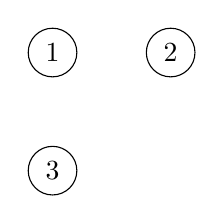
\begin{tikzpicture}[node distance={15mm}, main/.style = {draw, circle}] 
  \node[main] (1) {$1$};
  \node[main] (2) [right of=1] {$2$};
  \node[main] (3) [below of=1] {$3$};

  \end{tikzpicture}
  \caption{Wszystkie nieizomorficzne grafy 3-wierzchołkowe}
\end{figure}

W celu uniknięcia porównywania wszystkich grafów, do nowo dodanego grafu wyznaczane są orbity - tylko jeden sposób generacji każdego grafu spowoduje sytuację, gdzie nowo dodany wierzchołek znajduje się w pierwszej orbicie, co pozwala łatwo odrzucać izomorfizmy.

   \subsection{Generowanie grafów Ramseya}
   Generowanie grafów obarczonych ograniczeniami co do rozmiarów klik oraz zbiorów niezależnych wygląda niemal tak samo jak generowanie grafów dowolnych, 
   ale zawiera dodatkowy krok - sprawdzenie czy graf nie zawiera kliki lub zbioru niezależnego stopnia który zaburzyłby jego ramseyowskość. Takie grafy można odrzucać, ze względu na następujące twierdzenie:
     \begin{theorem}
      Jeżeli graf G posiada klikę stopnia n, oraz istnieje graf H taki że G jest podgrafem H, to H również posiada klikę stopnia n.
   \end{theorem}
  Dzięki powyższemu twierdzeniu wiemy, że wszelkie próby rozszerzenia grafu posiadającego klikę stopnia n powodują powstanie grafów z kliką przynajmniej tak wielkiego stopnia. Analogiczne rozumowanie można przeprowadzić wobec rozszerzania grafów ze zbiorem niezależnym o określonym stopniu. Dzięki temu odrzucanie grafów nieramseyowskich na wczesnym etapie generacji nie powoduje wykluczenia żadnych pożądanych grafów wyższych rzędów. Takie odrzucanie znacznie zmniejsza ilość grafów powstających na kolejnych etapach generacji, zwłaszcza dla grafów wyższego rzędu, bez czego wygenerowanie nawet grafów wymaganych do sklejania byłoby trudne. Nieizomorficznych grafów 17-wierzchołkowych jest ponad $10^{26}$\cite{OEIS}. Dzięki wczesnym wykluczaniu dla R(4,4) generowany jest tylko jeden taki graf. 
  
Odrzucanie grafów nieramseyowskich przy każdym rozszerzeniu pozwala wprowadzić dodatkową optymalizację. Jeżeli rozszerzymy graf o ograniczonym stopniu kliki lub zbioru niezależnego, to nowopowstały graf może mieć jedynie klikę lub zbiór niezależny łamiący ograniczenia jeżeli nowo dodany wierzchołek jest ich częścią. Wynikająca z tego mniejsza liczba wymaganych kontroli ramseyowośći uzyskać dalsze przyspieszenie algorytmu generacji grafów.
